\documentclass{article}
\usepackage[utf8]{inputenc}
\usepackage{graphicx}
\usepackage{hyperref}

\title{CSI 5387 Data Mining and Concept Learning Assignment 3}
\author{Lingfeng Zhang 300134245}
\date{March 2020}

\begin{document}

\maketitle

In this assignment, I use Python with scikit-learn package to handle it.

GitHub Source Code:

\href{https://github.com/RichardChangCA/CSI-5387-Data-Mining-and-Concept-Learning/tree/master/Assignment_3}{\url{https://github.com/RichardChangCA/CSI-5387-Data-Mining-and-Concept-Learning/tree/master/Assignment_3}}

All source codes, results, \LaTeX source codes and report are stored in this GitHub link.

\section{Part A: Association Analysis}

\subsection{(a)}

For minimum support of 0.5\% and minimum confidence of 50\%, there are too many generated rules, all results can be seen in file "results\_5.txt"(antecedent\_len=2) and "results\_5\_new.txt"(antecedent\_len=1).

Below lists several rules with top 10 highest lift with descending lift(antecedent length is 2):

1. 'curd', 'tropical fruit' -- 'yogurt'

2. 'whipped/sour cream', 'pip fruit' -- 'other vegetables'

3. 'onions', 'root vegetables' -- 'other vegetables'

4. 'citrus fruit', 'root vegetables' -- 'other vegetables'

5. 'tropical fruit', 'root vegetables' -- 'other vegetables'

6. 'butter', 'whipped/sour cream' -- 'other vegetables'

7. 'tropical fruit', 'whipped/sour cream' -- 'other vegetables'

8. 'butter', 'tropical fruit' -- 'other vegetables'

9. 'fruit/vegetable juice', 'root vegetables' -- 'other vegetables'

10. 'whole milk', 'onions' -- 'other vegetables'

If antecedent length is 1, only 1 rule can be generated.

'baking powder' -- 'whole milk'

\subsection{(b)}

For minimum support of 0.1\% and minimum confidence of 50\%, the better lift rule is:

Antecedent length = 2, they share the same highest lift:

'yogurt', 'rice' -- 'other vegetables'

'yogurt', 'rice' -- 'whole milk'

'yogurt', 'rice' -- 'root vegetables'

Antecedent length = 1: 

'honey' -- 'whole milk'

All results can be seen in file "results\_1.txt"(antecedent\_len=2) and "results\_1\_new.txt"(antecedent\_len=1).

\subsection{(c)}

If I were a marketing manager, I will choose rule "honey--whole milk" because minimum support is 0.1\% is sufficient and this rule's lift is the highest.

In addition, if the minimum support is higher, the algorithm may filter some useful rules. Moreover, the higher lift means the higher association between antecedents and consequent.

\subsection{Part B Clustering}

\subsection{1)}

\subsubsection{a)}

initialization:

C\_1:[[1, 0], [2, 1]]

C\_2:[[0, 1], [3, 3]]

sum\_squared\_error:7.5

kmeans iteration 1:

C\_1:[[1, 0], [0, 1], [2, 1]]

C\_2:[[3, 3]]

sum\_squared\_error:2.6666666666666665

\subsubsection{b)}

kmeans iteration 2:

C\_1:[[1, 0], [0, 1], [2, 1]]

C\_2:[[3, 3]]

sum\_squared\_error:2.6666666666666665

In iteration 2, kmeans algorithm reaches its optimal solution because MSE do not change anymore.

\subsection{2)}

For Hierarchical clustering algorithm, there are many linkage methods, such as complete, single, average, weighted and etc. More detail please check \href{https://docs.scipy.org/doc/scipy/reference/generated/scipy.cluster.hierarchy.linkage.html#scipy.cluster.hierarchy.linkage}{\url{https://docs.scipy.org/doc/scipy/reference/generated/scipy.cluster.hierarchy.linkage.html#scipy.cluster.hierarchy.linkage}} , which is a clickable link.

For this assignment, I just used complete and single linkage method.

For distance or dissimilarity matrix, single linkage method use formula:

$d(u,v) = min(dist(u[i],v[i]))$

, and complete linkage method use formula:

$d(u,v) = max(dist(u[i],v[i]))$

On the contrary, for similarity matrix, single linkage method use formula:

$d(u,v) = max(dist(u[i],v[i]))$

, and complete linkage method use formula:

$d(u,v) = min(dist(u[i],v[i]))$

,because similarity matrix can be simply equal to 1 minus dissimilarity matrix.

The steps to build up Dendrogram are shown below(In this case, I used similarity method and min method(complete) as linkage:

The similarity matrix is shown below:

\begin{center}
\begin{tabular}{ c c c c c c}

 & P0 & P1 & P2 & P3 & P4 \\

P0 & 1.00 & 0.10 & 0.41 & 0.55 & 0.35 \\

P1 & 0.10 & 1.00 & 0.64 & 0.47 & 0.98 \\
 
P2 & 0.41 & 0.64 & 1.00 & 0.44 & 0.85 \\ 
 
P3 & 0.55 & 0.47 & 0.44 & 1.00 & 0.76 \\
 
P4 & 0.35 & 0.98 & 0.85 & 0.76 & 1.00

\end{tabular}
\end{center}

The highest similarity value except 1.00 is 0.98, corresponding to P1 \& P4. We combine P1 and P4 together.

MIN[(P0,P1P4)] = MIN[(P0,P1),(P0,P4)] = MIN[0.1,0.35] = 0.1

MIN[(P2,P1P4)] = MIN[(P2,P1),(P2,P4)] = MIN[0.64,0.85] = 0.64

MIN[(P3,P1P4)] = MIN[(P3,P1),(P3,P4)] = MIN[0.47,0.76] = 0.47

\begin{center}
\begin{tabular}{ c c c c c}

 & P0 & P1P4 & P2 & P3 \\

P0 & 1.00 &  &  &  \\

P1P4 & 0.10 & 1.00 &  &  \\
 
P2 & 0.41 & 0.64 & 1.00 &  \\ 
 
P3 & 0.55 & 0.47 & 0.44 & 1.00 \\

\end{tabular}
\end{center}

The highest similarity value except 1.00 is 0.64, corresponding to P2 \& P1P4. We combine P2 and P1P4 together.

MIN[(P0,P1P4P2)] = MIN[(P0,P1P4),(P0,P2)] = MIN[0.1,0.41] = 0.1

MIN[(P3,P1P4P2)] = MIN[(P3,P1P4),(P3,P2)] = MIN[0.47,0.44] = 0.44

\begin{center}
\begin{tabular}{ c c c c}

 & P0 & P1P4P2 & P3 \\

P0 & 1.00 &  &  \\

P1P4P2 & 0.10 & 1.00 &  \\
 
P3 & 0.55 & 0.44 & 1.00 \\

\end{tabular}
\end{center}

The highest similarity value except 1.00 is 0.55, corresponding to P0 \& P3. We combine P0 and P3 together.

MIN[(P1P4P2,P0P3)] = MIN[(P1P4P2,P0),(P1P4P2,P3)] = MIN[0.1,0.44] = 0.1

\begin{center}
\begin{tabular}{ c c c}

 & P0P3 & P1P4P2 \\

P0P3 & 1.00 & \\

P1P4P2 & 0.10 & 1.00\\

\end{tabular}
\end{center}

Finally, combine P0P1P2P3P3 together as a whole cluster.

The whole procedure is shown below:

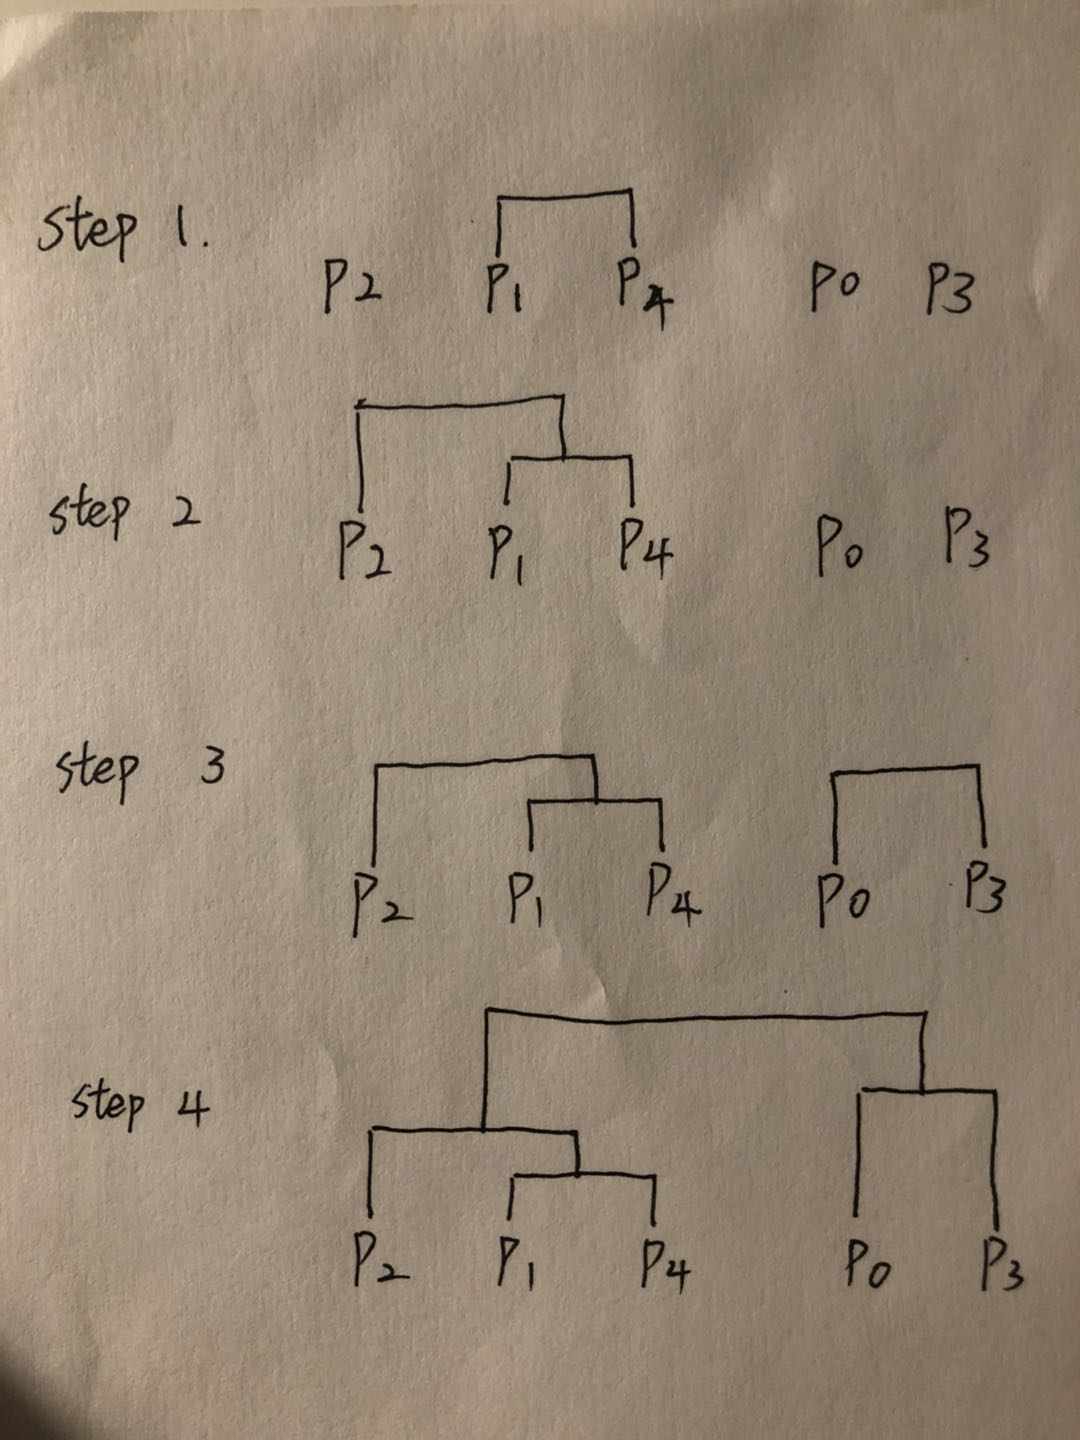
\includegraphics[scale=0.2]{steps.jpeg}

I used Agglomerative algorithm to do clustering task, and chose cluster number as 2,3,4 and 5 separately, and the linkage method is complete.

I got the clustering results below:

2 clusters: [0 1 1 0 1]

3 clusters: [2 0 0 1 0]

4 clusters: [2 0 3 1 0]

5 clusters: [2 4 3 1 0]

These results match up the result of Dendrogram.

The finial Dendrogram graph is shown below(linkage is complete):

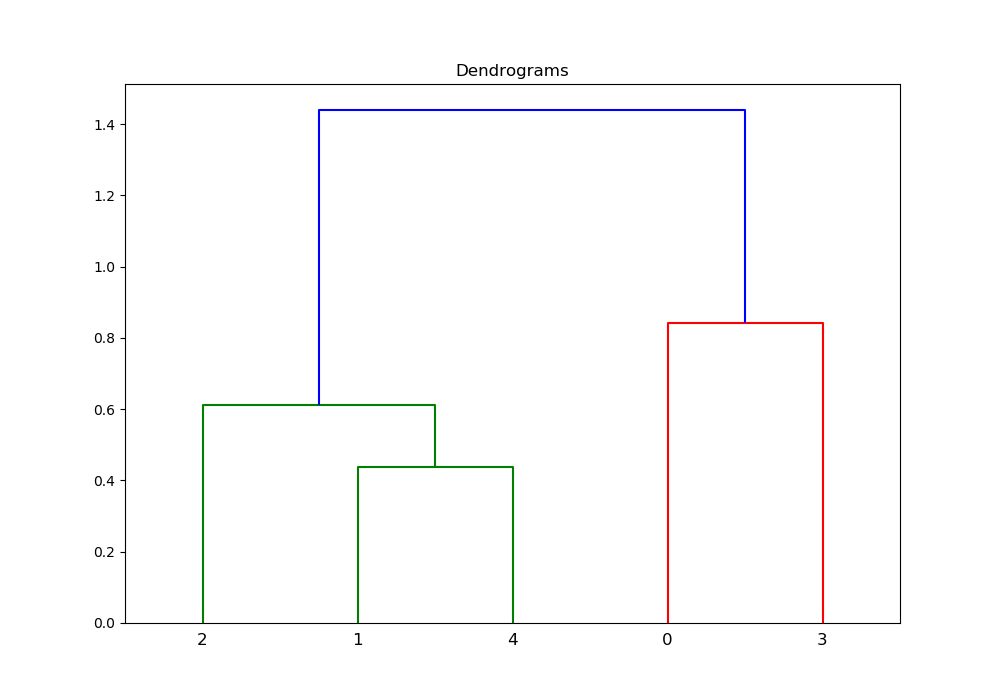
\includegraphics[scale=0.4]{Dendrograms.png}

If I replace the linkage method with single(max for similarity matrix), the Dendrogram is shown below:

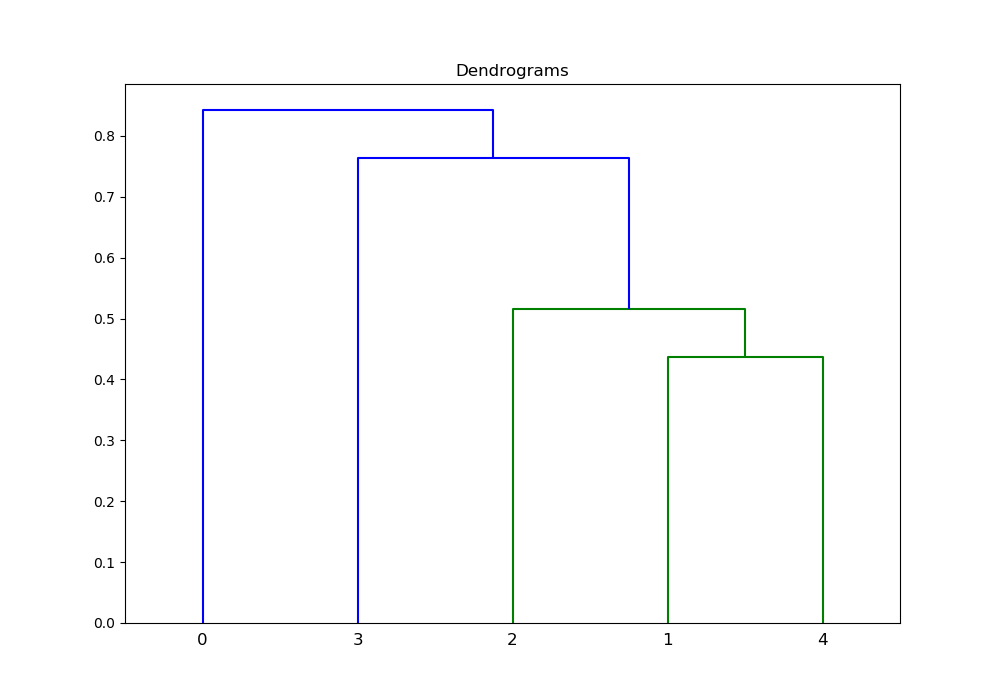
\includegraphics[scale=0.4]{Dendrograms_single.png}

\subsection{3)}

In DBSCAN algorithm, use similarity threshold of 0.8 (using the similarity matrix) or eps of 0.2 (for the dissimilarity matrix) as hyper-parameter because dissimilarity matrix can be simply equal to 1 minus similarity matrix(eps = 1 - similarity threshold).

By using DBSCAN method from sklearn.cluster, I got the results below(according to sklearn package):

clustering.labels\_ : [-1 -1 -1 -1 -1]

clustering.core\_sample\_indices\_ : [ ](empty)

,shows no core point and all of them are noise points because noisy samples are given the label -1.

Border points are points that are (in DBSCAN) part of a cluster, but not dense themselves (i.e. every cluster member that is not a core point). In this case, no border point.

If I set up eps as 0.5 the result is(according to sklearn package):

clustering.labels\_ : [-1  0 -1 -1  0]

clustering.core\_sample\_indices\_ : [1 4]

Core points are P1(second point) and P4(5-th point), others are noise points and no border point.

The similarity matrix is shown below:

\begin{center}
\begin{tabular}{ c c c c c c}

 & P0 & P1 & P2 & P3 & P4 \\

P0 & 1.00 & 0.10 & 0.41 & 0.55 & 0.35 \\

P1 & 0.10 & 1.00 & 0.64 & 0.47 & 0.98 \\
 
P2 & 0.41 & 0.64 & 1.00 & 0.44 & 0.85 \\ 
 
P3 & 0.55 & 0.47 & 0.44 & 1.00 & 0.76 \\
 
P4 & 0.35 & 0.98 & 0.85 & 0.76 & 1.00

\end{tabular}
\end{center}

similarity threshold is 0.8 and MinPts $\geq$ 2, I got results manually shown below:

P0: 1.00, noise

P1: 1,00,0.98, core

P2: 1.00,0.85, core

P3: 1.00, noise

P4: 0.98,0.85,1.00, core

I am confused why results are different and I can make sure the sklearn package is used properly.

\subsection{4)}

\subsubsection{a)}

The elbow plot is shown below:

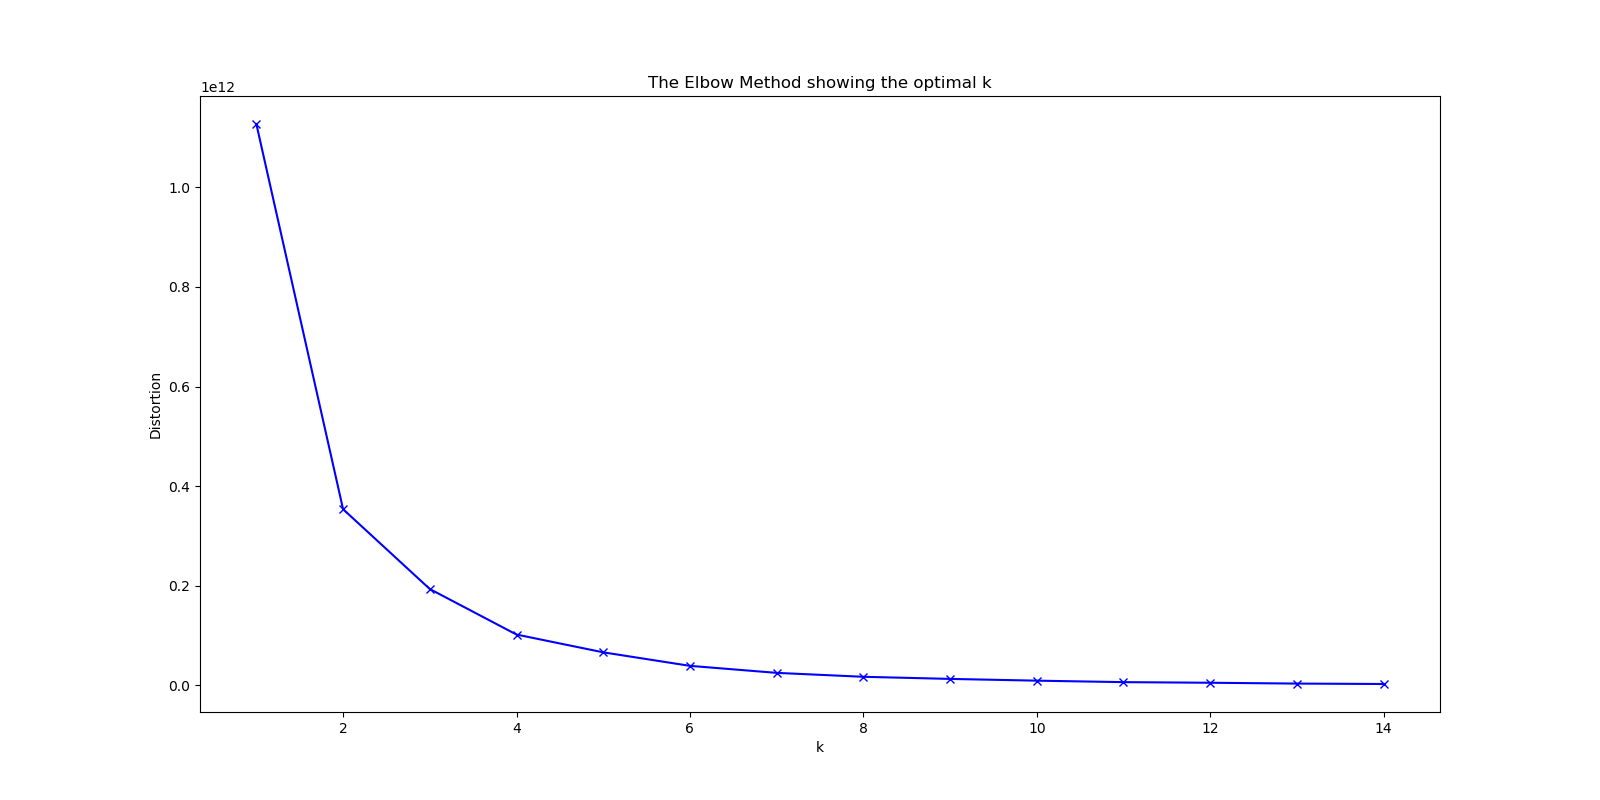
\includegraphics[scale=0.3]{elbow.png}

we can see the optimal number of clusters k using the elbow method is 11.

\subsubsection{b)}

By using sklearn.preprocessing.MinMaxScaler() method to standardize the attributes, the data distribution by using k-means clustering method is shown below:

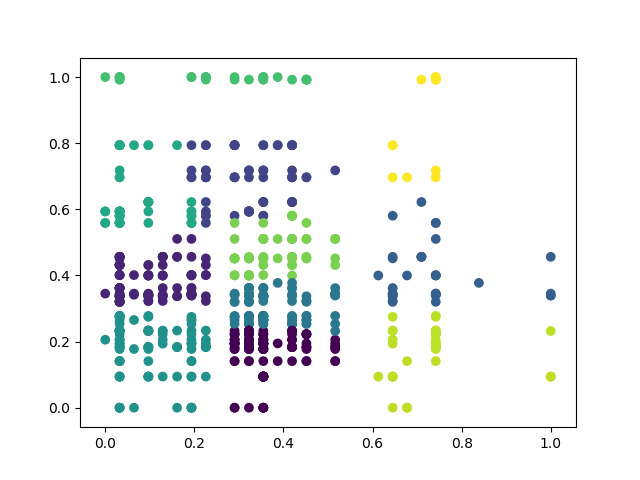
\includegraphics[scale=0.6]{data_scatter_plot.png}

\subsection{c)}

the data distribution by using agglomerative clustering with single linkage is shown below:

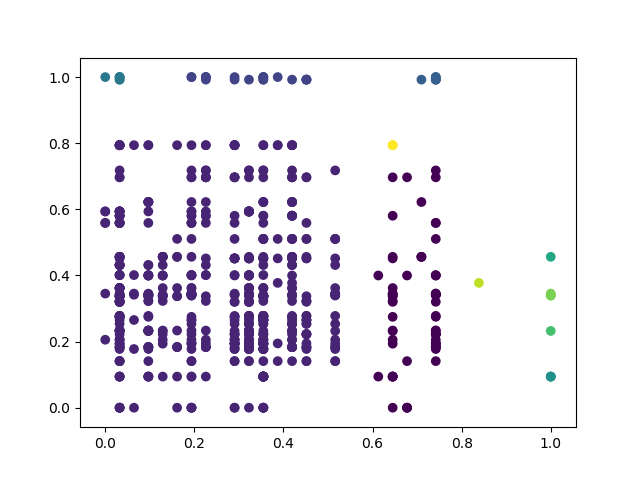
\includegraphics[scale=0.6]{AgglomerativeClustering_plot.png}

\subsubsection{d)}

the data distribution by using EM Gaussian mixture model is shown below:

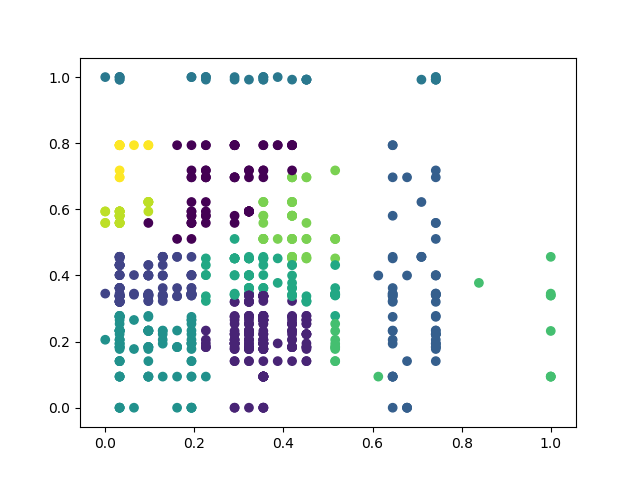
\includegraphics[scale=0.6]{EM_GaussianMixture_plot.png}

\subsection{e)}

In practice, the k-means algorithm is very fast (one of the fastest clustering algorithms available), but it falls in local minima. That’s why it can be useful to restart it several times. K-means clustering tends to find clusters of comparable spatial extent, while the expectation-maximization mechanism allows clusters to have different shapes. However, the performance of k-means is usually not as competitive as those of the other sophisticated clustering techniques because slight variations in the data could lead to high variance. Furthermore, clusters are assumed to be spherical and evenly sized, something which may reduce the accuracy of the K-means clustering Python results.

Agglomerative clustering algorithm is a bottom-up approach. Recursively merges the pair of clusters that minimally increases a given linkage distance. Start with many small clusters and merge them together to create bigger clusters.Once a decision is made to combine two clusters, it can’t be undone, and clustering speed is too slow for large data sets.

EM Gaussian mixture model satisfy statistical assumptions and more general than partitioning clustering.In addition, the clustering result of this mixture model looks reasonable.

EM Gaussian mixture model in this data distribution is more reasonable because k-means clustering algorithm may be sensitive to variance and the result of agglomerative clustering algorithm looks weird, the majority of points are clustered into a whole cluster and other points look like outliers.

\end{document}